%==============================================================================
% Matt Nichols' Homework Template
%==============================================================================


%Fill out this line with the homework number
\newcommand{\visibleusernames}
{\space man1, malesser, ac110 }
{}
\newcommand{\thisclass}{CSCI 160}
\newcommand{\thishw}{Final Project}

%==============================================================================
% Formatting parameters
%==============================================================================

\documentclass[11pt]{article}			% 11pt article
\author{Matt Nichols}
\date{\today}
\makeatletter					% Make '@' accessible.

%Fill out this line with your name and login
\def\@oddhead{\bf \thisclass \space - \thishw\hfill \visibleusernames} % Here they are

\oddsidemargin=0in				% Left margin minus 1 inch.
\evensidemargin=0in				% Same for even-numbered pages.
\textwidth=6.5in				% Text width (8.5in - margins).
\topmargin=0in					% Top margin minus 1 inch.
\headsep=0.2in					% Distance from header to body.
\textheight=8.5in					% Body height (incl. footnotes)
\skip\footins=4ex				% Space above first footnote.
\hbadness=10000					% No "underfull hbox" messages.
\makeatother					% Make '@' special again.

%==============================================================================
% Packages used
%==============================================================================

\usepackage{amsmath}				% want AMS fonts
\usepackage{amssymb}
%\usepackage{psfig}				% want to include EPS files
\usepackage[pdftex]{graphicx}				% for including images
\usepackage{algorithmic}
\usepackage{algorithm}
\usepackage{hyperref}
\usepackage{tikz}


%==============================================================================
% Macros
%==============================================================================
\newcommand{\new}[1]{{\em #1\/}}		% New term (set in italics).
\newcommand{\set}[1]{\{#1\}}			% Set (as in \set{1,2,3})
\newcommand{\setof}[2]{\{\,{#1} $\mid$~{#2}\,\}}	% Set (as in \setof{x}{x > 0})
\newcommand{\N}{\mathord{\Bbb N}}		% Positive integers.
\newcommand{\compl}[1]{\overline{#1}}		% Complement of ...            
\newcommand{\bigand}{\bigwedge}
\newcommand{\bigor}{\bigvee}
\newcommand{\OR}{\vee}
\newcommand{\AND}{\wedge}
\newcommand{\code}[1]{\texttt{#1}}
\newcommand{\nlogn}{n \log n}

\newcounter{qcounter}
\setcounter{section}{0}
\def\thesection{Section \arabic{section}}


% \begin{list}{b\alph{qcounter}.}{\usecounter{qcounter}} <-- helpful

%==============================================================================
% Title
%==============================================================================

\begin{document}
\centerline{\bf \LARGE\thishw: Knock Detection Entry System}
\centerline{\today}

\section{Introduction}
 % Introduce your project. Succinctly explain your problem and solution. Why did you choose to work on it?
Carrying keys around has always been a hassle for all of us. If one loses a key, he or she has to be assisted by someone else to get in to the room. A lot of times, there are situations where you wouldn't want to bring your keys with you either, such as when you're going on a run. I personally have forgotten my keys in my room, or have been locked out by my roommate numerous times. We wanted an easier way to enter and exit a locked room, and not ever have to worry about being locked out. 

Our project is a reasonably straightforward Arduino program which enables pulling a door handle down from the inside of a door once a specific pattern of knocks has been detected. This pattern is configurable via a ``record" function, and, when powered, the device is always listening for the pattern, ready to trigger a motor to open the door. If an incorrect knock pattern is given, the program alerts you through a buzz in the speaker. This way, the room is secure and you'll never be locked out because you don't have the key.

\section{Architecture}
% Describe the architecture of your system. Figures are welcomed and encouraged

\subsection{Hardware Design}

This program assumes a hardware configuration that includes a piezo element for knock sensing (connected on \verb|piezo_pin|, in our code), two LEDs for control output, a button to trigger the recording mode, a servo (\verb|s1|, connected on \verb|servo_pin|) to pull the deadbolt, and a second piezo speaker to buzz when an incorrect pattern is recognized, or the system times out (and starts waiting for another knock series).

The wiring of the system ended up being pretty straightforward (see diagram below). The piezo on the left is for audio output (signaling error events or a reset of the listening system) and the piezo on the right (highlighted in purple) is used for knock detection. The left (red) LED blinks whenever a knock is detected (mainly a debugging tool for us, though also helpful when the user is recording), and the right (green) LED is a control signal: it is turned on during recording, and is used to both signal a timeout event (reset of input knock pattern) and to replay a knock pattern to the user after it has been recorded. When the system receives a correct knock pattern, it will rotate the servo 180 degrees (enough to pull down a door handle or draw back a deadlock), wait a few seconds, and then rotate back to its original position. The rest of our hardware implementation is reasonably simple, but is diagrammed in full below.

\begin{center}
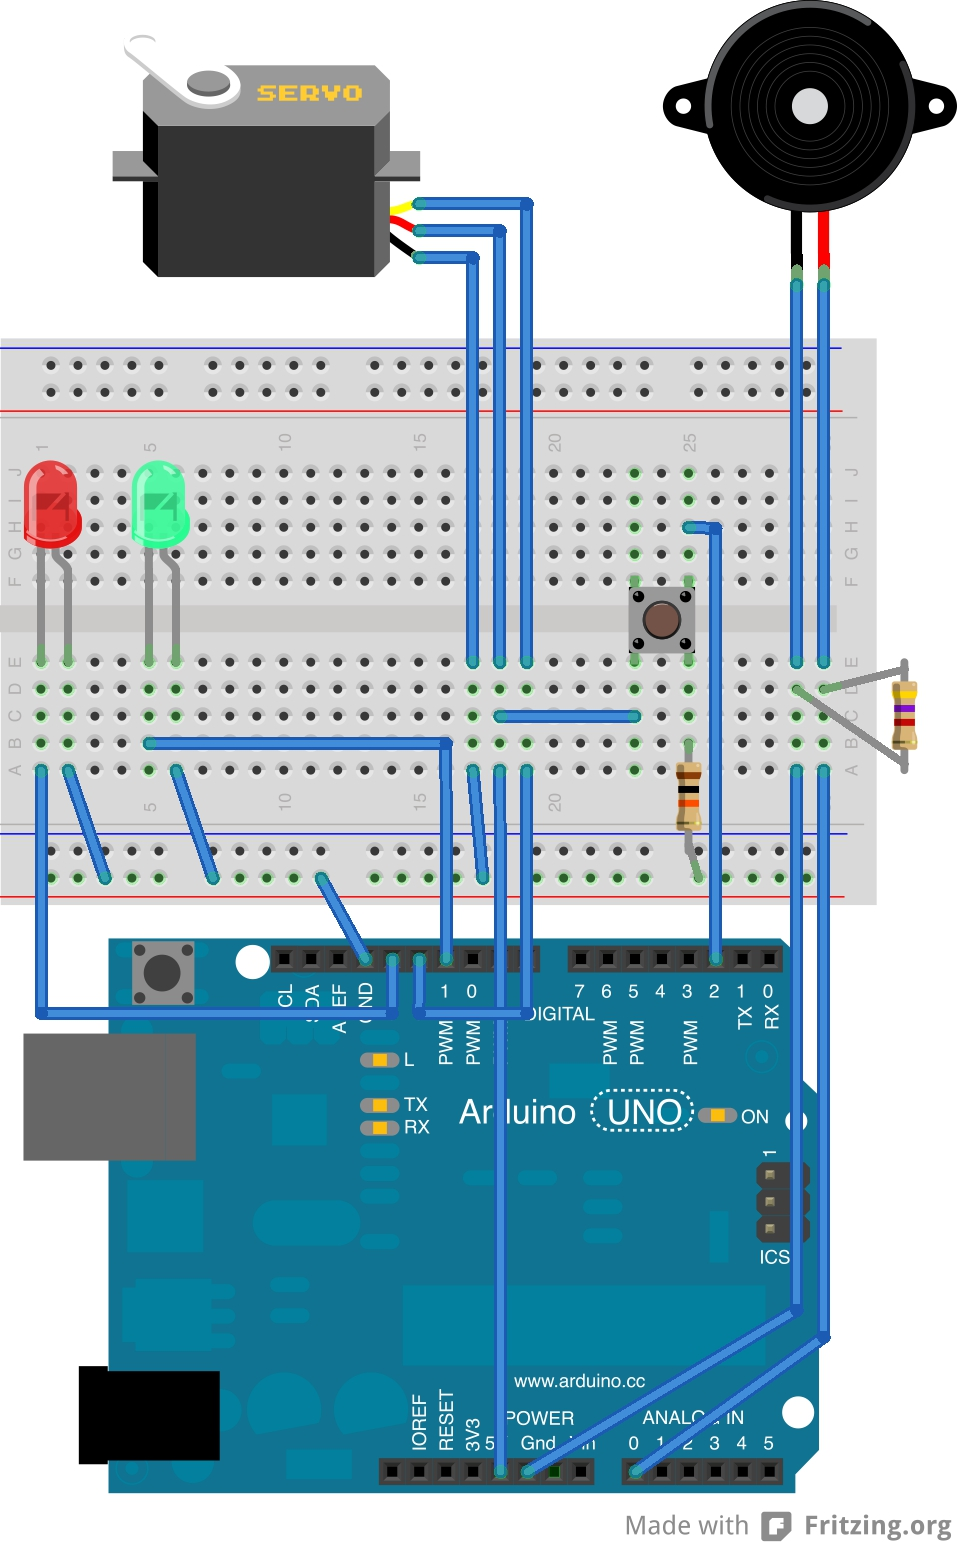
\includegraphics{knock_diagram_img.png}
\end{center}

\subsection{Software Design}

Left to describe is the operation of our software which is running on the Arduino, which is strictly procedural and adheres to a predetermined flow (i.e. we do not make use of interrupts on the Arduino platform).

The basic operation of our software can be summed up well as a finite state machine (below). The system's default state is iterating within the Arduino main loop, waiting for either a button press or a knock. At both \verb|Input| and \verb|Record|, it will continue listening for subsequent knocks, though the transitions out of these states are different: at \verb|Input|, it will only move on to evaluation of the knock pattern once \verb|n knocks| (the number of knocks in the current valid pattern) have been detected, while at \verb|Record|, it will wait for a timeout (i.e. knocking has stopped) or until the user has input the maximum allowable number of knocks to progress to the next state. Along both the \verb|timeout| and \verb|incorrect| edges, a sound will be played on the speaker. The \verb|Print| state corresponds to a blocking process during which the current valid pattern is echoed in appropriately spaced blinks on the control LED, and after this completes, it returns to its normal resting state. The rest of the system's operation within the state diagram should be self-explanatory, though we delve into a few more details (outside of the FSM) below.

\begin{center}
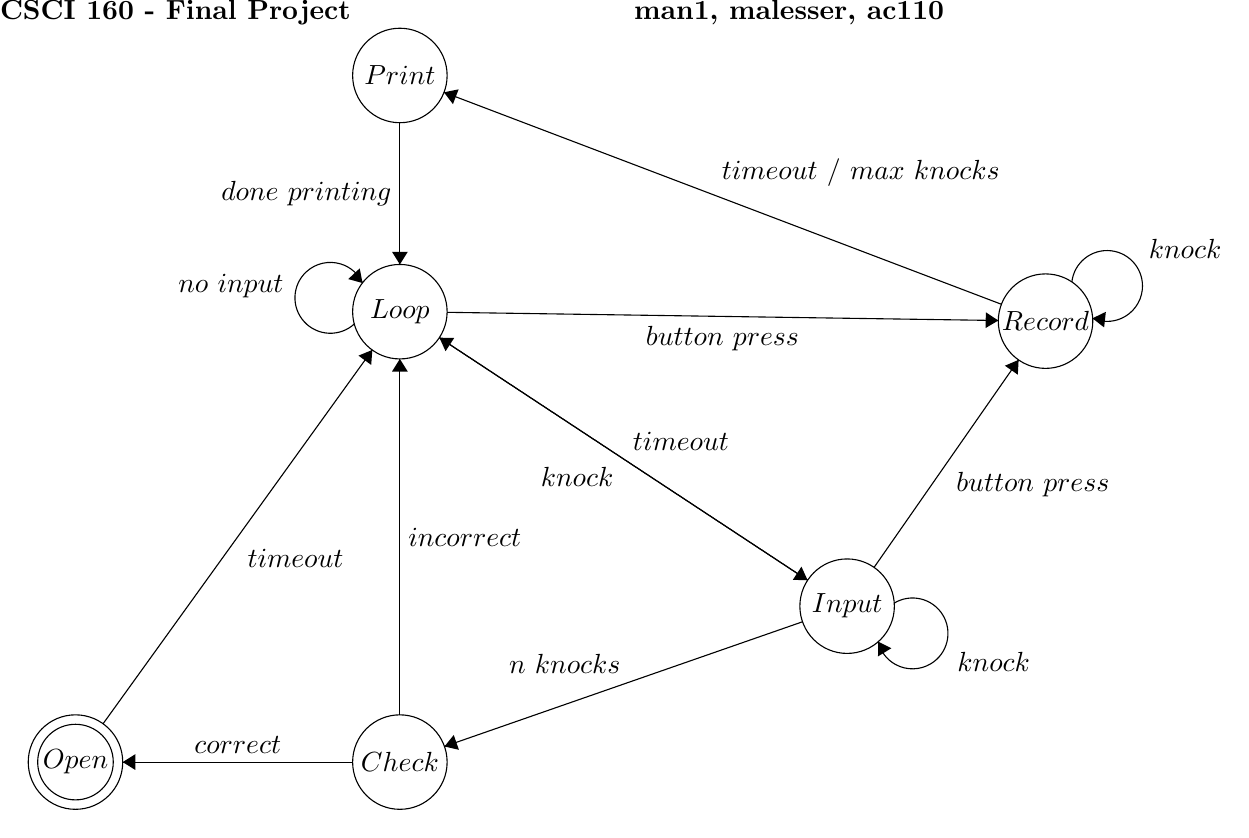
\begin{tikzpicture}[scale=0.2]
\tikzstyle{every node}+=[inner sep=0pt]
\draw [black] (26.6,-22.6) circle (3);
\draw (26.6,-22.6) node {$Loop$};
\draw [black] (55,-41.3) circle (3);
\draw (55,-41.3) node {$Input$};
\draw [black] (67.6,-23.2) circle (3);
\draw (67.6,-23.2) node {$Record$};
\draw [black] (26.6,-51.2) circle (3);
\draw (26.6,-51.2) node {$Check$};
\draw [black] (6,-51.2) circle (3);
\draw (6,-51.2) node {$Open$};
\draw [black] (6,-51.2) circle (2.4);
\draw [black] (26.6,-7.6) circle (3);
\draw (26.6,-7.6) node {$Print$};
\draw [black] (29.6,-22.64) -- (64.6,-23.16);
\fill [black] (64.6,-23.16) -- (63.81,-22.64) -- (63.79,-23.64);
\draw (47.08,-23.48) node [below] {$button\mbox{ }press$};
\draw [black] (29.11,-24.25) -- (52.49,-39.65);
\fill [black] (52.49,-39.65) -- (52.1,-38.79) -- (51.55,-39.63);
\draw (37.85,-32.45) node [below] {$knock$};
\draw [black] (23.713,-23.373) arc (312.7283:24.7283:2.25);
\draw (19.24,-20.97) node [left] {$no\mbox{ }input$};
\fill [black] (24.23,-20.78) -- (24.05,-19.85) -- (23.32,-20.53);
\draw [black] (52.49,-39.65) -- (29.11,-24.25);
\fill [black] (29.11,-24.25) -- (29.5,-25.11) -- (30.05,-24.27);
\draw (44.45,-31.45) node [above] {$timeout$};
\draw [black] (52.17,-42.29) -- (29.43,-50.21);
\fill [black] (29.43,-50.21) -- (30.35,-50.42) -- (30.02,-49.48);
\draw (37.07,-45.62) node [above] {$n\mbox{ }knocks$};
\draw [black] (23.6,-51.2) -- (9,-51.2);
\fill [black] (9,-51.2) -- (9.8,-51.7) -- (9.8,-50.7);
\draw (16.3,-50.7) node [above] {$correct$};
\draw [black] (57.982,-41.109) arc (121.40093:-166.59907:2.25);
\draw (61.97,-44.82) node [right] {$knock$};
\fill [black] (56.97,-43.55) -- (56.96,-44.49) -- (57.81,-43.97);
\draw [black] (26.6,-48.2) -- (26.6,-25.6);
\fill [black] (26.6,-25.6) -- (26.1,-26.4) -- (27.1,-26.4);
\draw (27.1,-36.9) node [right] {$incorrect$};
\draw [black] (7.75,-48.77) -- (24.85,-25.03);
\fill [black] (24.85,-25.03) -- (23.97,-25.39) -- (24.78,-25.98);
\draw (16.89,-38.28) node [right] {$timeout$};
\draw [black] (64.8,-22.13) -- (29.4,-8.67);
\fill [black] (29.4,-8.67) -- (29.97,-9.42) -- (30.33,-8.48);
\draw (55.86,-14.69) node [above] {$timeout\mbox{ }/\mbox{ }max\mbox{ }knocks$};
\draw [black] (26.6,-10.6) -- (26.6,-19.6);
\fill [black] (26.6,-19.6) -- (27.1,-18.8) -- (26.1,-18.8);
\draw (26.1,-15.1) node [left] {$done\mbox{ }printing$};
\draw [black] (69.27,-20.722) arc (173.74488:-114.25512:2.25);
\draw (74.12,-18.63) node [right] {$knock$};
\fill [black] (70.58,-23.02) -- (71.32,-23.6) -- (71.43,-22.61);
\draw [black] (56.71,-38.84) -- (65.89,-25.66);
\fill [black] (65.89,-25.66) -- (65.02,-26.03) -- (65.84,-26.6);
\draw (61.9,-33.61) node [right] {$button\mbox{ }press$};
\end{tikzpicture}
\end{center}

The device begins with a default knock pattern of ten equally spaced knocks. In our system, an $n$ knock pattern is represented as a $n-1$ sized array, each element being the ratio between adjacent knocks (so the default knock pattern is represented as $[1, 1, 1, 1, 1, 1, 1, 1, 1]$). When the system hears a first knock, it will begin recording the time offsets between subsequent knocks, and after it receives the number of expected knocks, relative ratios are calculated from the recorded offsets. Each of these ratios are then compared to those of the current key pattern (within an error margin), and if they all match then the servo is triggered and the deadbolt is pulled open.

Recording is very similar: pressing the button triggers record mode, and then the current key pattern will be replaced by whatever ratioed pattern is recorded after the button press (and before a timeout, as stated). This pattern will then be played back to the user on a LED (as mentioned above), and the device will re-enter normal operation, listening for entry attempts. If fewer than three knocks are recorded during this process, the valid key pattern will not be replaced, and the previously (and still) valid key pattern will be what is played back on the LED.

\subsection{Conceptual}

Following is a basic overview for how we imagine an end user approaching the operation of our device. After the above explanation, these things may be evident, but consider this the higher-level, more conceptual, usability-oriented side of our design. 

\textbf{Installation:} the device must be installed such that the piezo is pressed directly against the door, to best register knocking. The servo should be configured to pull the deadbolt or door handle when it rotates.

\textbf{Recording:} press the button once, and then knock out the desired pattern on the inside of the door. Wait for the timeout, and then make sure the replayed pattern (on the second, lower LED) is as you desire. Your patterns must consist of between three and ten knocks (inclusive); shorter knock patterns will not overwrite the current key pattern, and recording will cut off after ten knocks.

\textbf{Unlocking:} simply knock the pre-recorded pattern on the outside of the door, and if the time ratios between your knocks match the stored key pattern, the servo will pull the deadlock or door handle. It must be manually re-locked afterwards. If you make a mistake in the pattern, wait four seconds (the timeout) and try again.

\section{Implementation}
% Challenges, etc.
Timeout: We chose a timeout of 4 seconds. From a user standpoint, we decided it was the right amount of time because 4 seconds between knocks is too long for a pattern, and isn't so long that the user would get impatient waiting for it to timeout.

Threshold: We have a threshold of 0.5. This means that the most any interval between knocks can be wrong by is 0.5. For example, if the interval between 2 knocks is 3, a "correct" input is anywhere from 2.5 to 3.5. After multiple trials we discovered that this constant was the perfect error margin for a standard user.

Knock threshold: This threshold sets how loud a knock has to be in order to be registered. We chose 3 because it detects most knocks, and no static.

Keeping door open: The door stays open for 3 seconds, and nothing can happen with the program for 2 seconds after it closes. The door stays open that long because it's the right amount of time to give the user to enter. We had to block the program for 2 seconds after it closes becasue it would mess up the circuit voltages.

Max number of knocks: We limited the user to a maximum number of 10 knocks for their pattern. We chose this number because it allows for creativity and unique knocking patterns. We limited it to 10 because longer knock patterns would result in the user forgetting the pattern.

Debounce-delay: The sensor doesn't detect a knock as a singular event. It will detect a singular knock as many knocks that happen 
extremely close together. We need a debounce delay to make the program wait to make sure the program doesnt think the vibrations after the knock are more knocks. We chose .1 seconds because you would never try to do two knocks that quickly, and it fixes the problem stated.


\section{Evaluation}
% did it work? Are there any corner cases? How would you solve them?
We were able to successfully connect the finished product to a door.  The piezo sensor used to detect knocks is fairly cheap, so sometimes knocks are not detected correctly, but it works fairly well.  To get the best results, the components must be placed somewhere in the center of the door so that all vibrations are picked up clearly.  

Recording and playback of patterns works perfectly, and with the addition of a piezo speaker it is easy to tell when you haven't correctly knocked out the pattern, or your knocks have timed out.  One problem with the finished product is that the servo we purchased only is able to turn 180 degrees.  This means that it is only able to pull a doorknob or lock a small distance.  We were able to solve this problem by pre-pulling the knob a small amount, so that the knob only has to be pulled a small amount before the door is opened.

One edge case to deal with is ambient vibrations in the door that the system is connected to.  If it picks up stray vibrations, it could either mess up the patter the user is trying to knock out, or pick up knocks when the user isn't even using the device.  Luckily, the first problem is solved by merely re-knocking the pattern, as the buzzer lets you know when you have made a mistake.  If knocks are being picked up when the user isn't knocking at all, the buzzer will sound after a timeout, but nothing else will happen.

\section{Related Work}
% Are there any similar solutions? Compare yours to theirs, if possible.
There aren't many similar affordable solutions. Doors with fingerprint scanners exist but are extremely expensive, even though they're more secure. These go for around \$300.

``The Clapper" also exists, that gives current to an outlet if it detects claps. However, it doesn't let you customize the sequence of claps. It doesn't directly connect to a motor either. Lastly, it detects sound as a pose to vibrations. Our project won't detect random noises, only vibrations on the door whereas ``The Clapper" could interpret white noise and randomly open and close the door. ``The Clapper" goes for around \$20. 

Lockitron is a Kickstarter project that uses smart phones to lock and unlock doors. To use Lockitron, you first need to attach the Lockitron shell around your deadbolt. This shell is smart; it's connected to WiFi and has Bluetooth. From anywhere in the world, you can unlock or lock your door from your smartphone. You can also grant access to other users. Lockitron also automatically unlocks the door when you walk near it with your smartphone. With Lockitron, you would still either need your key or a phone to get into you're locked house. It doesn't entirely address the problem we were having. You can still lock your phone inside the house, and if you don't want to run with keys, why would you run with your phone. We need a solution that doesn't physically require any hardware, and Lockitron doesn't give us that. It also costs around \$200. The device can be pre-ordered at: \url{www.lockitron.com/preorder}

Our project's cost came out to around \$50. If we were to sell this project, our costs would decrease of bulk order so we could sell for around \$70 to turn a fairly significant profit.

\section{Future Work}
% Describe here features that you wanted to implement, but due to time/resource constraints you weren't able to.

If we had had the time, our first stretch goal for this project was to implement remote unlocking via SMS messaging. The basic idea here would be to send a text to a specific number with a control command (eg. ``open'' or ``close''), and if this message originates from a verified number the command would be executed on the device. This could work well as both an override (if we forget the pattern), as well as a good way to let friends into a room which you're not in, et cetera.

We managed to write the backend (i.e. server code) for this aspect of the application, though didn't have time to implement the hardware and Arduino code side of this system. In the \verb|remote_unlock/| directory of our repo and project handin, we have a script which runs as a Twilio endpoint (see \url{www.twilio.com}), and also has a route to advertise the current (intended) state of the device. Assuming we had our board hooked up to an ethernet connection from which we could access the server, it would be simple to poll against \verb|[server port]/state| and trigger the servo when the "Unlocked" state is observed.

Two further improvements which could be made to our device are making it battery powered (currently it must be connected to a laptop or a wall socket at all times) and having audio as well as visual playback for echoing recorded patterns.

\end{document}